\documentclass[a4paper,12pt,oneside,pdflatex,italian,final,twocolumn]{article}

\usepackage[utf8]{inputenc}
\usepackage{parallel}
\usepackage{siunitx}
\usepackage{booktabs}
\usepackage{fancyhdr}
\usepackage{subcaption}
\usepackage{minted}
\usepackage{hyperref}
\usepackage{pdfpages}

\usepackage[export]{adjustbox}
\usepackage[margin=0.5in]{geometry}
\addtolength{\topmargin}{0in}

\usepackage{libertine}
\renewcommand*\familydefault{\sfdefault}  %% Only if the base font of the document is to be sans serif
\usepackage[T1]{fontenc}

\hypersetup{
	colorlinks=true, %set true if you want colored links
	linktoc=all,     %set to all if you want both sections and subsections linked
	linkcolor=blue,  %choose some color if you want links to stand out
	urlcolor=blue,   %url color
}

\definecolor{LightGray}{gray}{0.95}

\title{Custom Minimum ECU}
\author{Achmadi ST MT}
\date{June 2023}

\begin{document}
	\pagestyle{fancy}
	
	\lhead{Achmadi}
	\chead{\today}
	\rhead{Specification Document}
	
	\onecolumn
	
	\begin{figure}
		
	\end{figure}\begin{minipage}{0.47\textwidth}
		\centering
		
	\end{minipage}
	\hfill
	\begin{minipage}{0.47\textwidth}
		\raggedleft
		\Huge \textbf{Custom Minimum ECU v0.1}
	\end{minipage}

	\begin{figure}
		\begin{minipage}{0.47\textwidth}
			
			\section{Overview}
			\begin{itemize}
				\item Minimal and Flexible Engine Control Unit
				\item Reading TPS and RPM with calibration capability
				\item Control Injection and Ignition 
				\item Serial Data Interface in Real-time
				\item Designed to easy of use for general Injection engines
				\item Build as shield board top ST-Nucleo64 with STM32F103RBT6 chip
			\end{itemize}
			
		\end{minipage}
		\hfill
		\begin{minipage}{0.47\textwidth}
			\centering
			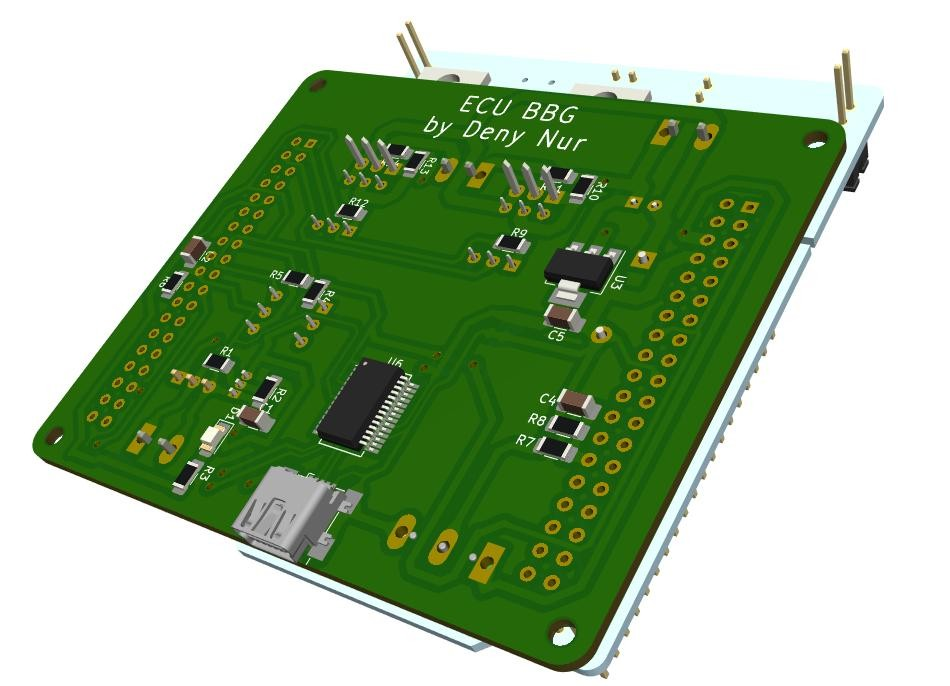
\includegraphics[width=0.7\textwidth,right]{images/mockup.jpg}
			
		\end{minipage}
	\end{figure}

	\raggedright

	\section{Repository URLs}
	
	\begin{itemize}
		\item PCB Design: \url{https://github.com/deninur2427/ecu_pnm/tree/main/circuits/ecupnm_nucf103rb/}
		
		\item Firmware: \url{https://github.com/deninur2427/ecu_pnm/tree/main/firmware/}
		
		\item Interface: \url{https://github.com/deninur2427/ecu_pnm/tree/main/interface/ecu_view/}
		
		\item Overall Repository: \url{https://github.com/deninur2427/ecu_pnm/}
	\end{itemize}

	\section{Technical specification}
	\centering
	\begin{tabular}{lcr}
		\toprule
		Parts & Unit & Value \\
		\midrule
		Power voltage & $V$ & 12 \\
		Dimensions & $mm*mm*mm$ & xx*yy*zz (without cable) \\
		Weight & $g$ & x \\
		Main Chip & & STM32F103RBT6 \\
		Storage & & Internal EEPROM \\
		USB  Data Interface & & USB-Serial FT232RL \\
		Engine Control Transistor & & IRF540N \\
		TPS Input & & 12-bit ADC \\
		PULSER Input & & Any pulsed signals \\
		\bottomrule
	\end{tabular}
	
	\raggedright
	
	\newpage
	\section{Unit Preview}
	
	\subsection{Shield Bottom}
	
	\begin{figure}[h]
		\centering
		\begin{subfigure}[b]{0.32\textwidth}
			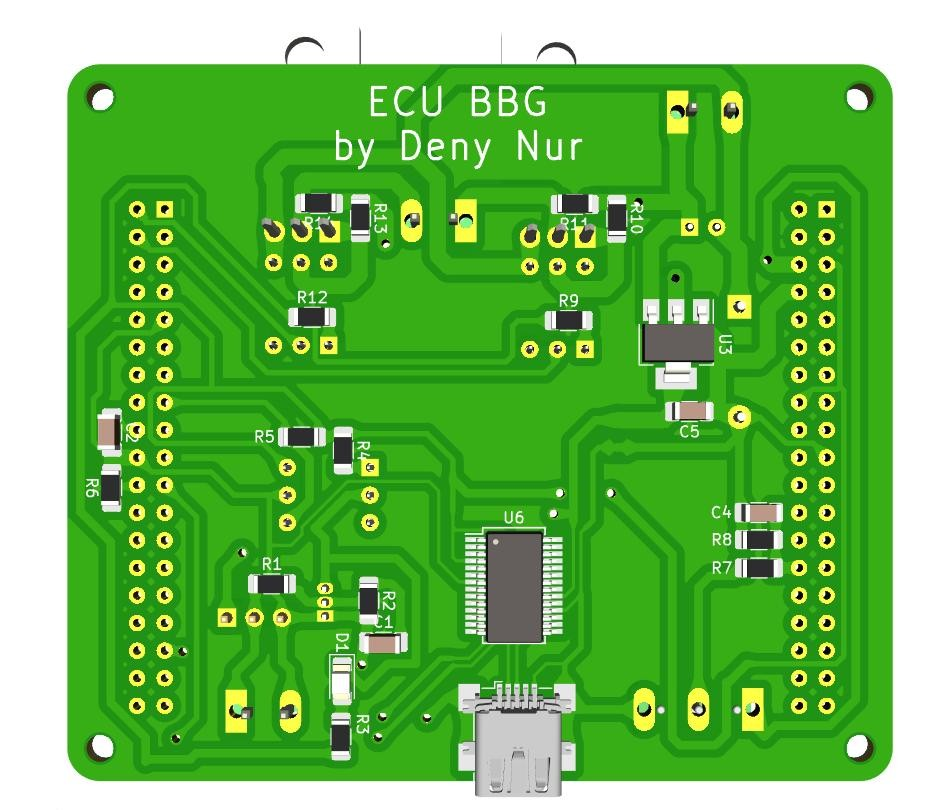
\includegraphics[width=\textwidth]{images/shield_bot.jpg}
			\caption{Mockup}
		\end{subfigure}
		~
		\begin{subfigure}[b]{0.32\textwidth}
			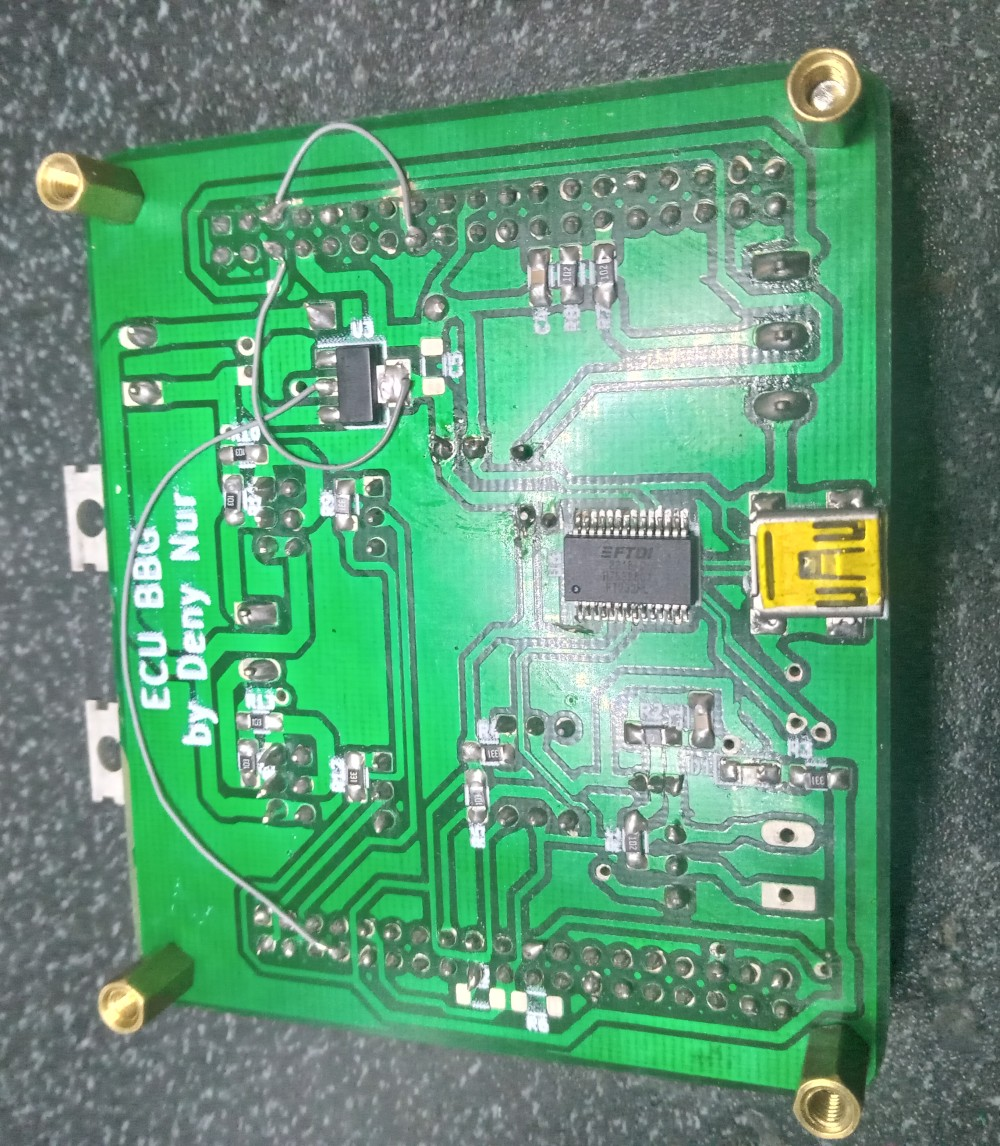
\includegraphics[width=0.7\textwidth,rotate=-90]{images/pcb_bot.jpg}
			\caption{Actual}
		\end{subfigure}
	\end{figure}

	\subsection{Top Bottom}
	
	\begin{figure}[h]
		\centering
		\begin{subfigure}[b]{0.32\textwidth}
			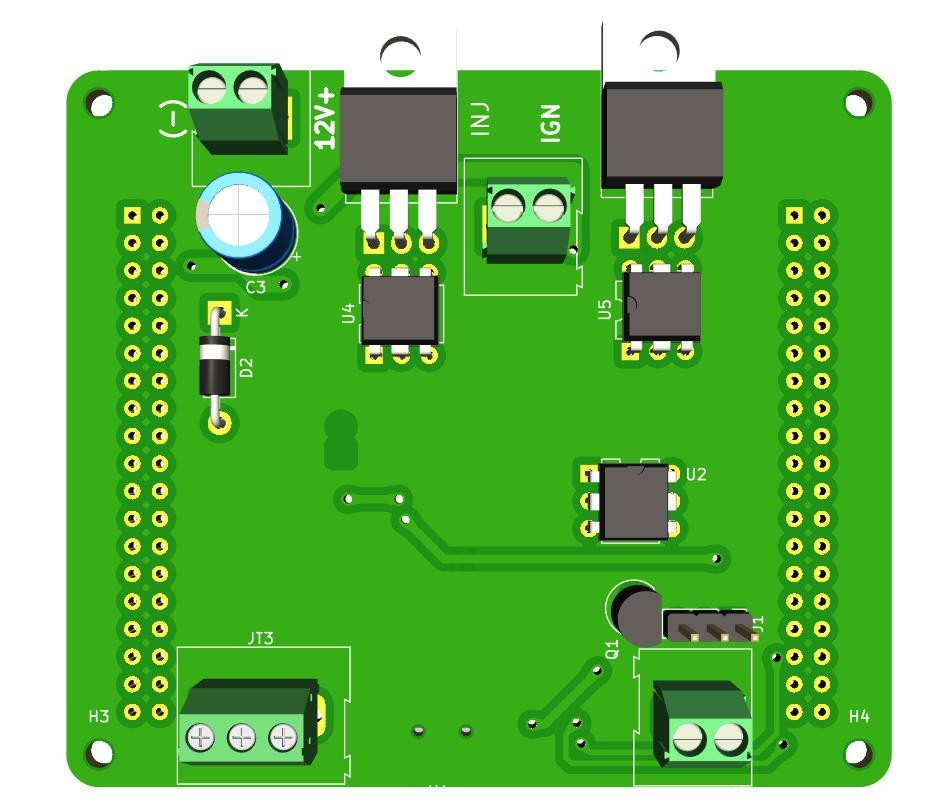
\includegraphics[width=\textwidth]{images/shield_top.jpg}
			\caption{Mockup}
		\end{subfigure}
		~
		\begin{subfigure}[b]{0.32\textwidth}
			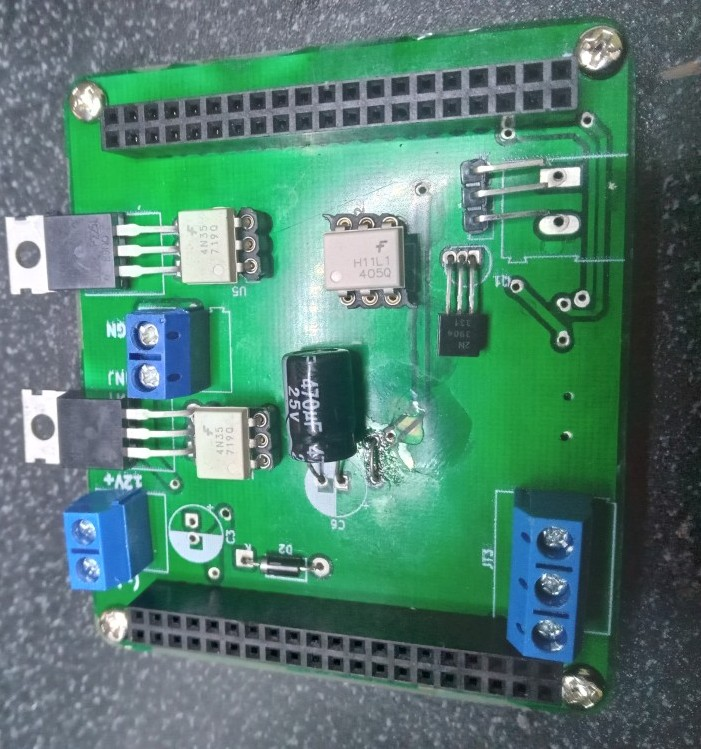
\includegraphics[width=0.7\textwidth,rotate=-90]{images/pcb_top.jpg}
			\caption{Actual}
		\end{subfigure}
	\end{figure}

	\subsection{Assembled Unit}
	
	\begin{figure}[h]
		\centering
		\begin{subfigure}[b]{0.32\textwidth}
			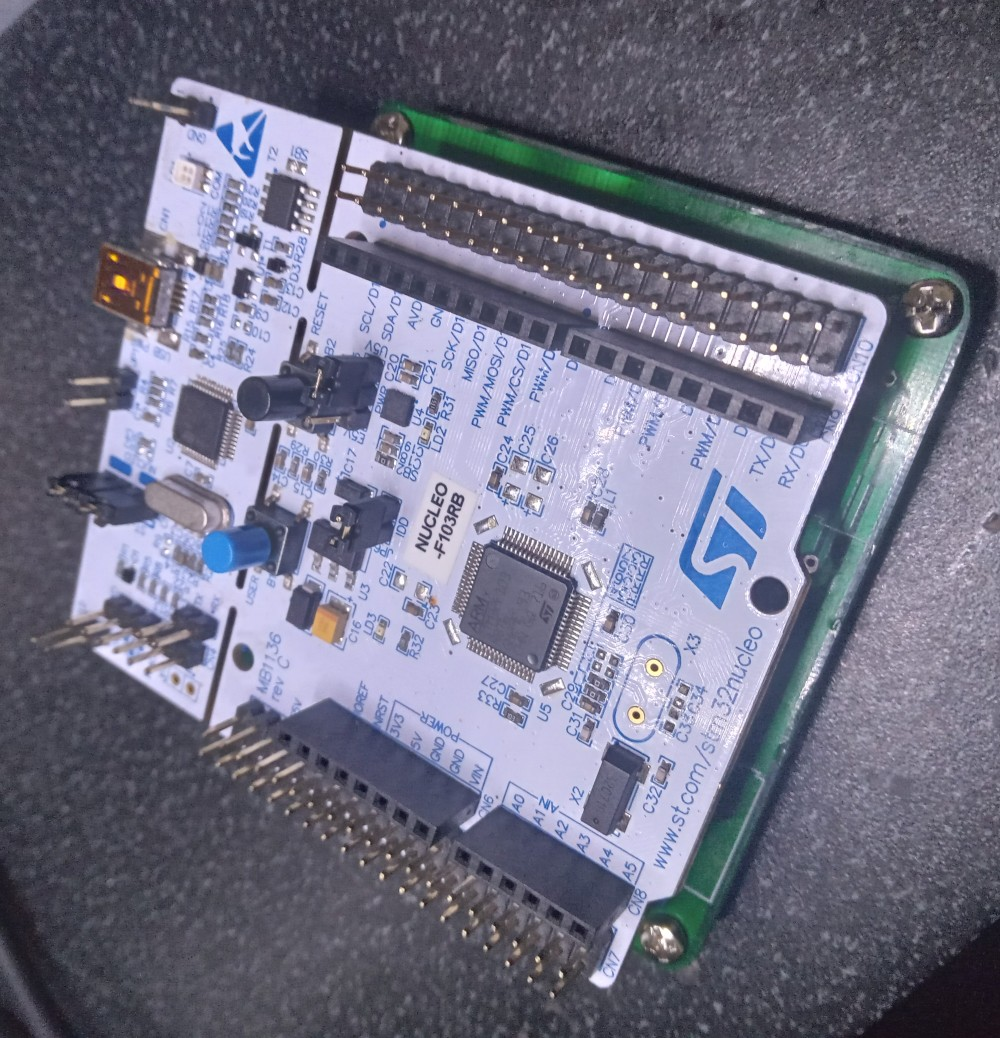
\includegraphics[width=0.7\textwidth]{images/unit_top.jpg}
			\caption{Unit Top}
		\end{subfigure}
		~
		\begin{subfigure}[b]{0.32\textwidth}
			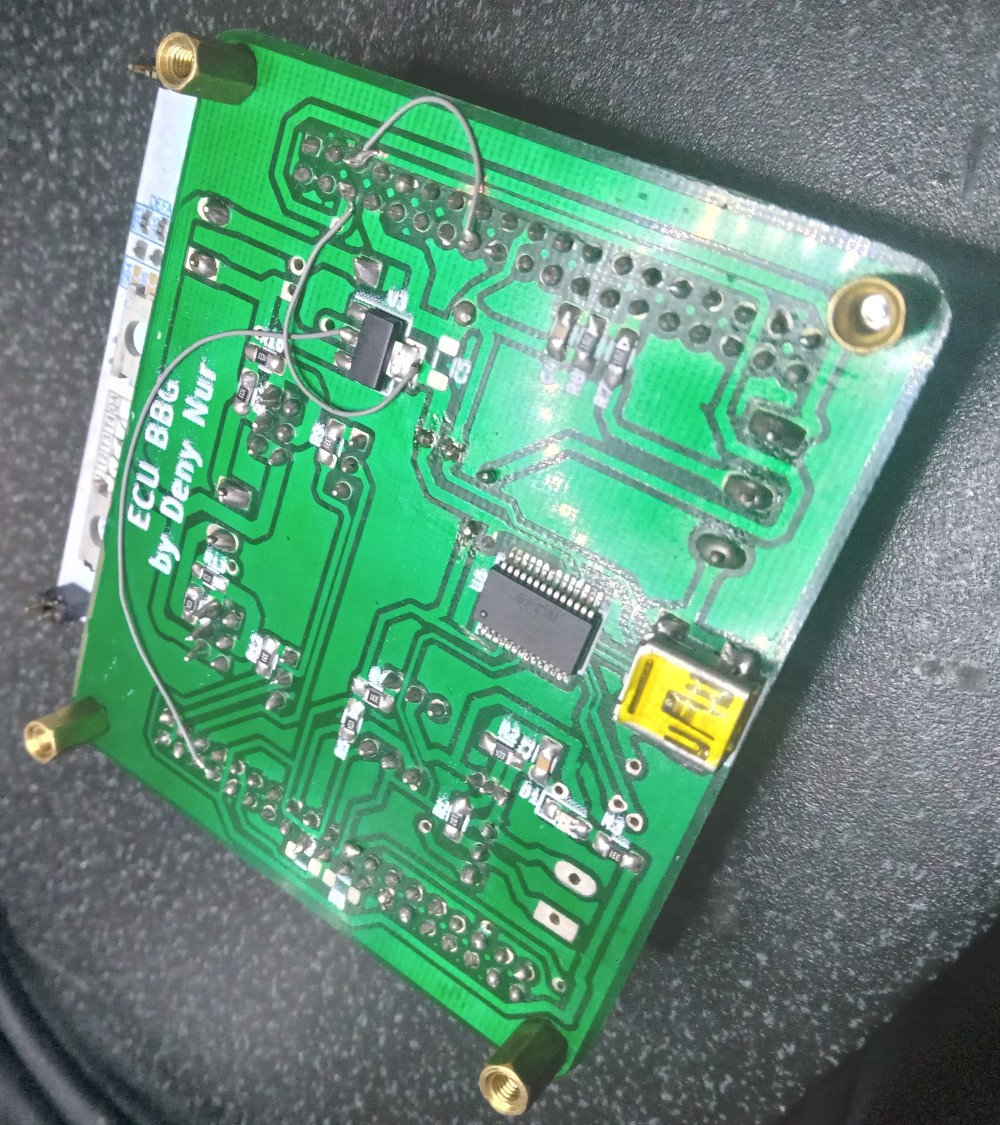
\includegraphics[width=0.7\textwidth]{images/unit_bot.jpg}
			\caption{Unit Bottom}
		\end{subfigure}
	\end{figure}

	\section{Schematic Design}
	
	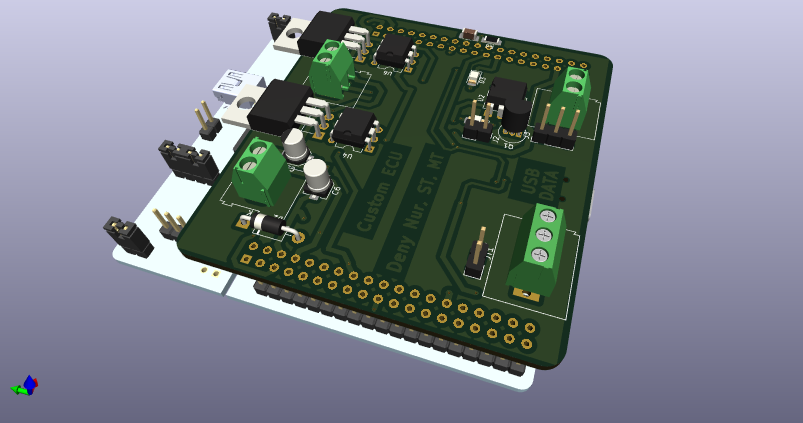
\includepdf[pages=-,angle=-90]{images/ecupnm_nucf103rb.pdf}
	
	\newpage
	\section{Firmware Summary}
	
	In Summary:
	\begin{itemize}
		\item Library Framework: ChibiOS/RT
		
		\item Running Mode: Real-Time Operating System
		
		\item Compiler target: GCC ARM with Newlib 
	\end{itemize}
	
	Some code snippet from \href[]{https://github.com/deninur2427/ecu_pnm/blob/main/firmware/ecu/main.c}{main.c}:
	
	\begin{minted}[frame=lines,framesep=2mm,fontsize=\normalsize,bgcolor=LightGray]{c}
int main(void) {
	// Hardware Abstraction Layer initialization
	halInit();
	
	// RTOS scheduler initialization
	chSysInit();
	
	// EEPROM initialization
	ecu_MEM_Init(); 
	
	// I/O Pins initialization
	ecu_GPIO_Init();
	
	// Serial Shell initialization
	ecu_SHELL_Init();
	
	// Input Capture initialization
	ecu_ICU_Init();
	
	// Analog-Digital initialization
	ecu_ADC_Init();
	
	// Generic Timer initialization
	ecu_GPT_Init();
	
	while (true) {
		// Serial Shell Loop initialization
		ecu_SHELL_Loop();
		
		// Latency to keep scheduling from race
		chThdSleepMilliseconds(500);
	}
}
	\end{minted}
	
	\section{Recommended Wiring Diagram}
	
	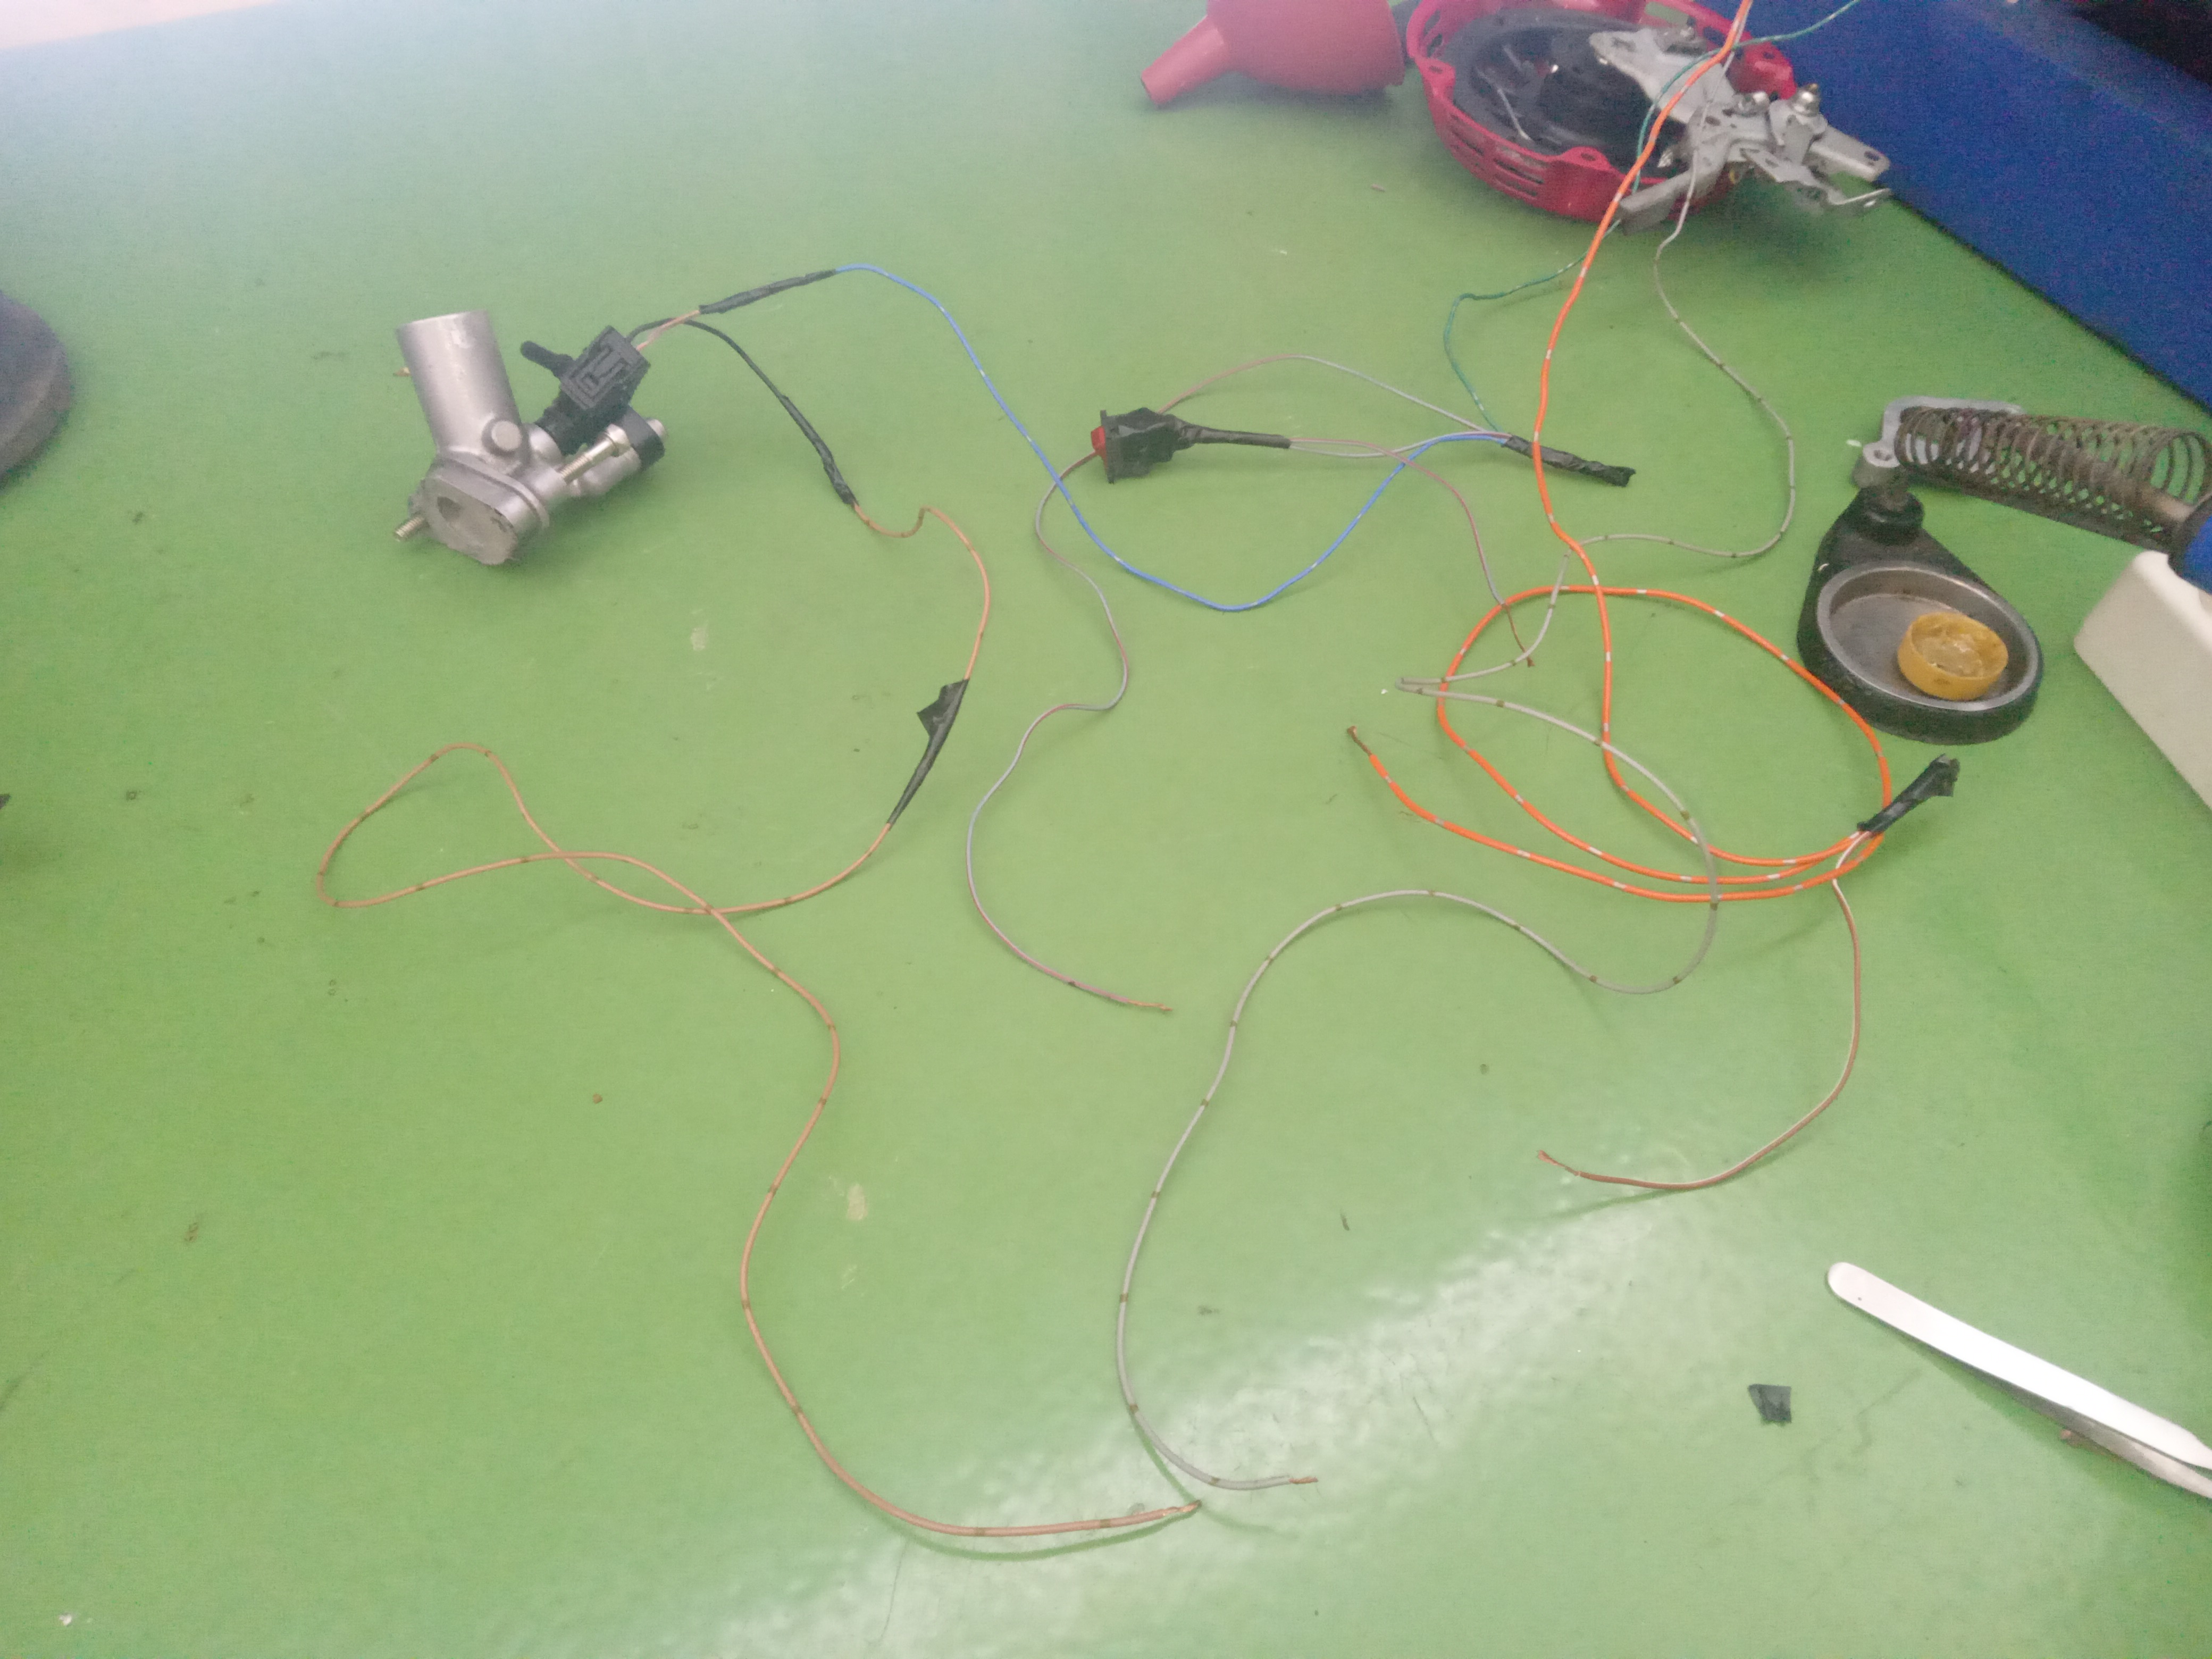
\includepdf[pages=-,angle=0]{images/wiring.pdf}
	
	\section{Interface Preview}
	
	In summary:
	\begin{itemize}
		\item Communicate with ECU through serial data
		
		\item Can Display engine throttle percent and RPM value in real-time
		
		\item Designed to manage Injection and Ignition mappings based on TPS-RPM
		
		\item Written in C++ and Qt5, compatible with Windows and GNU/Linux operating system
	\end{itemize}

	\subsection{Preview}
	
	\centering
	\begin{figure} [h]
		\centering
		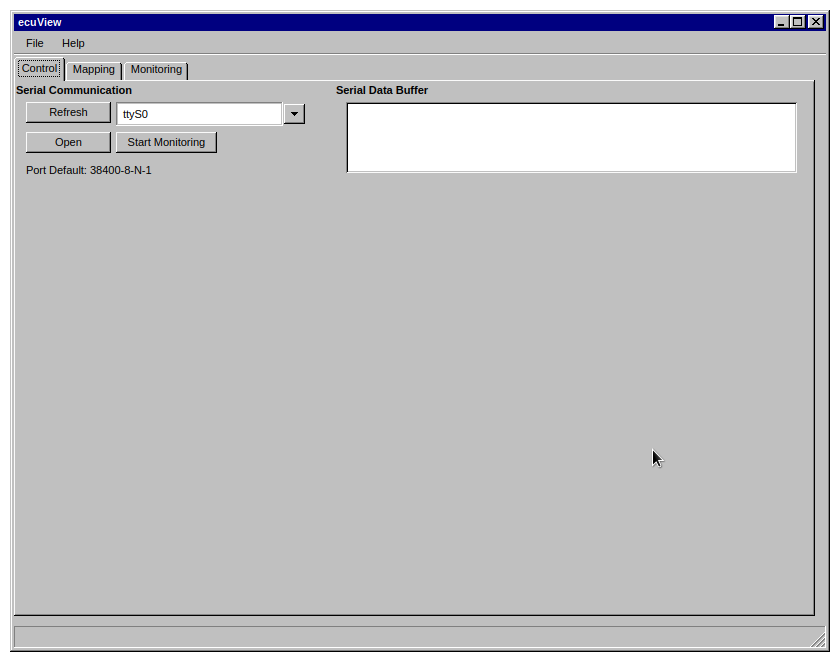
\includegraphics[width=0.55\textwidth,]{images/iface_main.png}
		\caption{Serial Data Control}
	\end{figure}
	
	\begin{figure} [h]
		\centering
		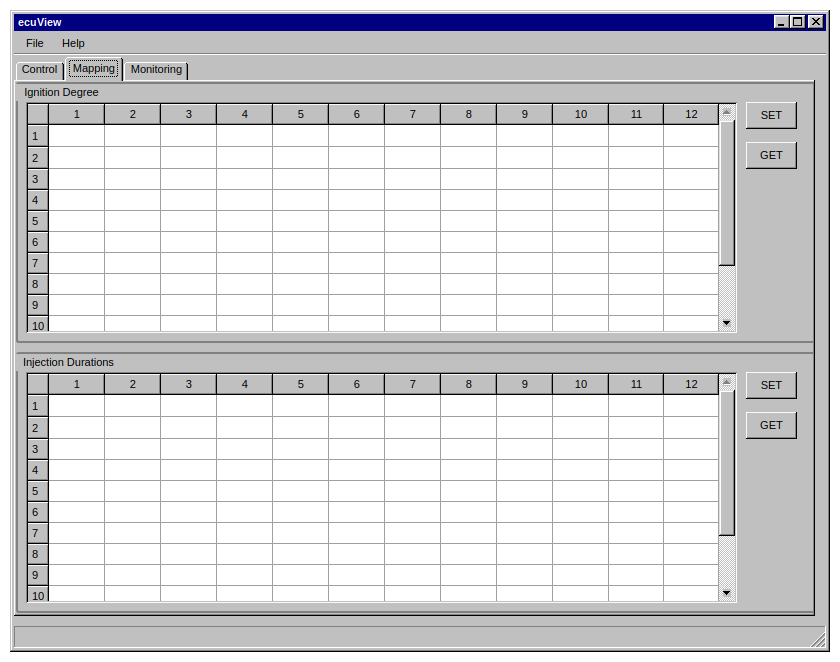
\includegraphics[width=0.55\textwidth,]{images/iface_map.png}
		\caption{Injection and Ignition Mapping}
	\end{figure}

	\newpage
	\begin{figure} [h]
		\centering
		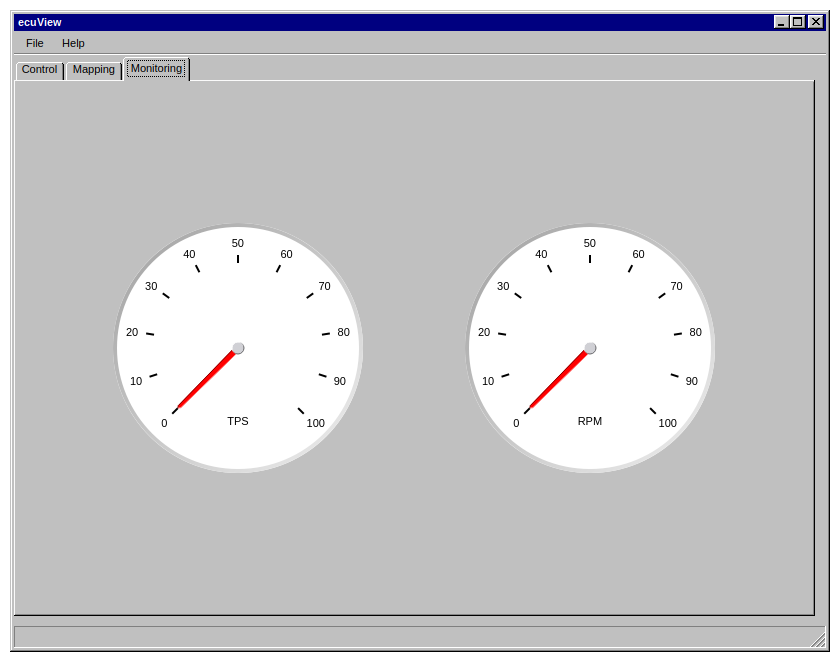
\includegraphics[width=0.55\textwidth,]{images/iface_dial.png}
		\caption{TPS and RPM Dial Monitoring}
	\end{figure}
	
	\raggedright
	\section{Assembled Parts}
	
	List of Assembled Parts:
	\begin{itemize}
		\item Custom Minimum Engine Control Unit prototype PCB
		
		\item ST Nucleo64 board with STM32F103RBT6 chip
		
		\item Mini USB Cables
		
		\item Acrylic Cranktooth in 12-miss-1 and 24-miss-1
	\end{itemize}

	\begin{figure} [h]
		\centering
		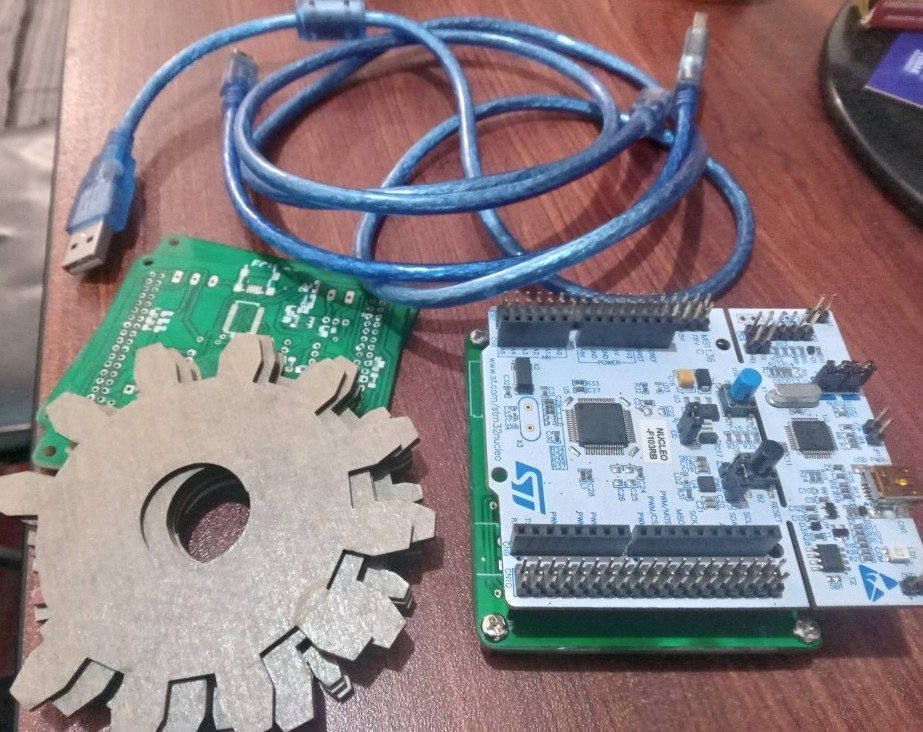
\includegraphics[width=0.55\textwidth,]{images/parts.jpg}
		\caption{Currently Assembled Parts}
	\end{figure}
\end{document}